%%%%%%%%%%%%%%%%%%%%%%%%%%%%%%%%%%%%%%%%%
% Short Sectioned Assignment
% LaTeX Template
% Version 1.0 (5/5/12)
%
% This template has been downloaded from:
% http://www.LaTeXTemplates.com
%
% Original author:
% Frits Wenneker (http://www.howtotex.com)
%
% License:
% CC BY-NC-SA 3.0 (http://creativecommons.org/licenses/by-nc-sa/3.0/)
%
%%%%%%%%%%%%%%%%%%%%%%%%%%%%%%%%%%%%%%%%%

%----------------------------------------------------------------------------------------
%	PACKAGES AND OTHER DOCUMENT CONFIGURATIONS
%----------------------------------------------------------------------------------------

\documentclass[paper=a4, fontsize=11pt]{scrartcl} % A4 paper and 11pt font size

\usepackage[T1]{fontenc} % Use 8-bit encoding that has 256 glyphs
\usepackage{fourier} % Use the Adobe Utopia font for the document - comment this line to return to the LaTeX default
\usepackage[english]{babel} % English language/hyphenation
\usepackage{amsmath,amsfonts,amsthm,amssymb} % Math packages

\usepackage{lipsum} % Used for inserting dummy 'Lorem ipsum' text into the template

\usepackage{sectsty} % Allows customizing section commands
\allsectionsfont{\centering \normalfont\scshape} % Make all sections centered, the default font and small caps

\usepackage{fancyhdr} % Custom headers and footers

% my packages
\usepackage{commath}
\usepackage{mathtools}
\usepackage{graphicx}
\usepackage{algorithm}
\usepackage[]{algpseudocode}
\DeclarePairedDelimiter{\ceil}{\lceil}{\rceil}
\usepackage{pgfplots}
\pgfplotsset{compat=newest}
\usepackage{hyperref}
\usepackage{enumitem}
\usepackage{caption}
\usepackage{subcaption}
\usepackage{multirow}
\usepackage{tkz-graph}
\usepackage{adjustbox}
\usepackage{cancel}
\usepackage[percent]{overpic}

\newlist{filedescription}{description}{2}
\setlist[filedescription]{font=\normalfont\normalcolor\bfseries\itshape}

\newlist{paramdescription}{description}{1}
\setlist[paramdescription]{font=\normalfont\normalcolor\itshape}

\pagestyle{fancyplain} % Makes all pages in the document conform to the custom headers and footers
\fancyhead{} % No page header - if you want one, create it in the same way as the footers below
\fancyfoot[L]{} % Empty left footer
\fancyfoot[C]{} % Empty center footer
\fancyfoot[R]{\thepage} % Page numbering for right footer
\renewcommand{\headrulewidth}{0pt} % Remove header underlines
\renewcommand{\footrulewidth}{0pt} % Remove footer underlines
\setlength{\headheight}{13.6pt} % Customize the height of the header

\numberwithin{equation}{section} % Number equations within sections (i.e. 1.1, 1.2, 2.1, 2.2 instead of 1, 2, 3, 4)
\numberwithin{figure}{section} % Number figures within sections (i.e. 1.1, 1.2, 2.1, 2.2 instead of 1, 2, 3, 4)
\numberwithin{table}{section} % Number tables within sections (i.e. 1.1, 1.2, 2.1, 2.2 instead of 1, 2, 3, 4)

\setlength\parindent{0pt} % Removes all indentation from paragraphs - comment this line for an assignment with lots of text

% new commands
\newcommand{\filename}[1]{\textbf{\textit{#1}}}
\newcommand{\funcname}[1]{\textbf{#1}}
\newcommand{\inv}{^{\raisebox{.2ex}{$\scriptscriptstyle-1$}}}
\renewcommand{\vec}[1]{\mathbf{#1}}

\makeatletter
\renewcommand*\env@matrix[1][*\c@MaxMatrixCols c]{%
  \hskip -\arraycolsep
  \let\@ifnextchar\new@ifnextchar
  \array{#1}}
\makeatother

\makeatletter
\def\BState{\State\hskip-\ALG@thistlm}
\makeatother

\DeclareMathAlphabet{\mathcal}{OMS}{cmsy}{m}{n}
\DeclareMathOperator*{\argmin}{arg\,min} % Jan Hlavacek

\newtheorem{theorem}{Theorem}
\newtheorem{definition}{Definition}

%----------------------------------------------------------------------------------------
%	TITLE SECTION
%----------------------------------------------------------------------------------------

\newcommand{\horrule}[1]{\rule{\linewidth}{#1}} % Create horizontal rule command with 1 argument of height

\title{	
\normalfont \normalsize 
\textsc{Mathematical foundations of computer graphics and vision} \\ [25pt] % Your university, school and/or department name(s)
\horrule{0.5pt} \\[0.4cm] % Thin top horizontal rule
\huge Exercise 6. Variational Methods and the Primal Dual Algorithm\\ % The assignment title
\horrule{2pt} \\[0.5cm] % Thick bottom horizontal rule
}

\author{Dongho Kang \\ \small 16-948-598} % Your name

\date{\normalsize May 28, 2017} % Today's date or a custom date

\begin{document}

\maketitle % Print the title

%----------------------------------------------------------------------------------------
%	README
%----------------------------------------------------------------------------------------

MATLAB R2016b version was used for coding and testing:

\begin{center}
MathWorks, MATLAB R2016b (9.1.0.441655) \\
64-bit (maci64) 
\end{center}

The \filename{code} directory contains the followings:

\begin{filedescription}
	\item [part2.m] script .m file for exercise part 2.
	\item [part3\_1.m] script .m file for exercise part 3, task 1.
	\item [part3\_2.m] script .m file for exercise part 3, task 2.
	\item [functions] directory which contains functions by me. 
	\item [Part 2 - Interactive Segmentation] provided directory with modified code.
	\item [Part 3 - Inpainting] provided directory with modified code.
\end{filedescription} 

\textbf{IMPORTANT:} Code implementation should be run by those scripts above only. Every custom function paths and parameters are only set in the script \filename{part2.m}, \filename{part3\_1.m} and \filename{part3\_2.m}. \\ 

In order to run each task program, go to the code directory and run script by MATLAB command \textit{part2}, \textit{part3\_1} or \textit{part3\_2}

\pagebreak

%----------------------------------------------------------------------------------------
%	PROBLEM 1
%----------------------------------------------------------------------------------------

\section{exercise part 1: Convexity of the Rudin Osher Fatemi Functional}

%----------------------------------------------------------------------------------------
%	TASK 1
%----------------------------------------------------------------------------------------
\subsection{Task 1: Proof of the convexity}

In this part, the following functions were checked if they are convex or not. 

\begin{itemize}
	\item $x \rightarrow \sin(x)$

\begin{figure}[H]
\vspace{-5mm}
\caption{$f(x) = \sin(x)$\label{fig:sinx}}
\centering
\noindent\makebox[\textwidth]{
  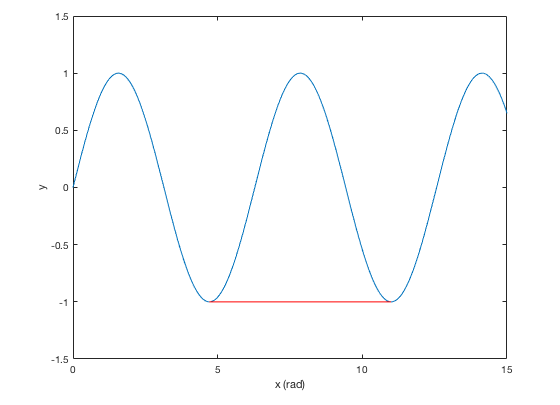
\includegraphics[width=\textwidth]{sinx.png}
}
\end{figure}
\textbf{$f(x) = \sin(x)$ is not a convex function.} Recall the definition of convex function: \\

\begin{definition} \label{def:convex}

A function $f: \mathcal{V} \rightarrow \mathbb{R}$ is called \textit{convex} if the function domain $\mathcal{V}$ is a convex set and if 
\begin{equation*}
	f(\lambda x + (1 - \lambda)y) \leq \lambda f(x) + (1 - \lambda) f(y) \qquad \forall x, y \in \mathcal{V} \quad \text{and} \quad 0 \leq \lambda \leq 1.
\end{equation*} 	
\end{definition}

For $\lambda = \frac{1}{2}$, $x = \frac{3}{2}\pi$ and $y = \frac{7}{2}\pi$, (as Figure \ref{fig:sinx})
\begin{align}
	f(\frac{3}{4}\pi + \frac{7}{4}\pi) = \sin(\frac{10}{4}\pi) = 1  \nleq \frac{1}{2} \, f(\frac{3}{4}\pi) + \frac{1}{2} \, f(\frac{7}{4}\pi) = \frac{1}{2} \, \sin(\frac{3}{4}\pi) + \frac{1}{2} \, \sin(\frac{7}{4}\pi) = 0
\end{align}

thus $f(x) = \sin(x)$ is not a convex function. 
	
%----------------------------------------------------------------------------------------
	\item $x$ $\rightarrow$ $x^2$

\begin{figure}[H]
\vspace{-5mm}
\caption{$f(x) = x^2$\label{fig:xsq}}
\centering
\noindent\makebox[\textwidth]{
  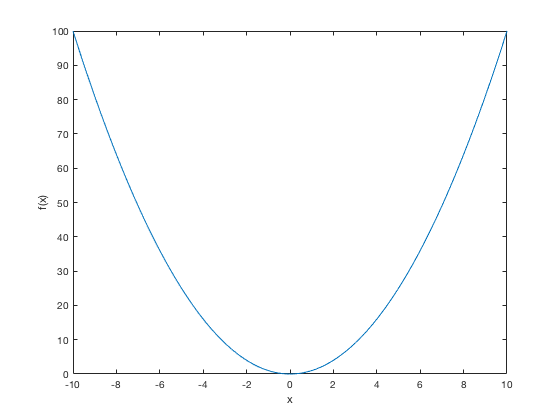
\includegraphics[width=\textwidth]{xsq.png}
}
\end{figure}

\textbf{$f(x) = x^2$ is a convex function.} \\

\begin{theorem}	\label{thm:firstorder}

First order condition: A differentiable function $f: \mathcal{V} \rightarrow \mathbb{R}$ is convex iff
\begin{equation}
	f(y) \geq f(x) + \nabla f(x)^T(y-x) \qquad \forall x, y \in \mathcal{V}
\end{equation}
\end{theorem}

By the theorem, for $f(x) = x^2$
\begin{align}
	f(x) + \nabla f(x)^T(y-x) &= x^2 + 2 x (y - x) \\
	&= x^2 + 2xy - 2x^2 \\
	&= 2xy - x^2 \\
	f(y) - f(x) - \nabla f(x)^T(y - x) &= y^2 - 2xy + x^2 \\ 
	&= (y - x)^2 \geq 0 \\
	\therefore 	f(y) \geq f(x) + \nabla f(x)^T(y-x) \label{eq:firstorder}
\end{align}

By (\ref{eq:firstorder}) and Theorem \ref{thm:firstorder}, $f(x) = x^2$ is a convex function. 
	
%----------------------------------------------------------------------------------------
	\item $x \rightarrow \sin(x) + x^2$ 

\begin{figure}[H]
\vspace{-5mm}
\caption{$f(x) = \sin(x) + x^2$\label{fig:sinxplusxsq}}
\noindent\makebox[\textwidth]{
  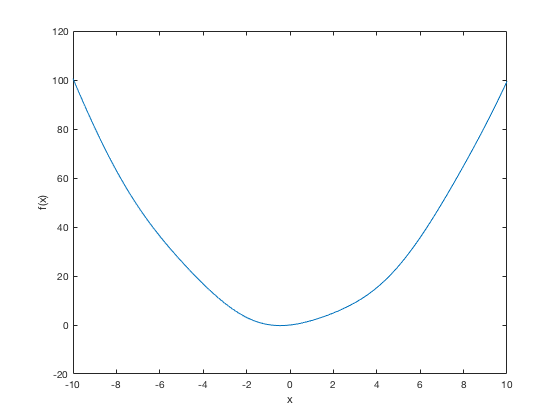
\includegraphics[width=\textwidth]{sinxplusxsq.png}
}
\end{figure}

\textbf{$f(x) = \sin(x) + x^2$ is a convex function.} Here is a proof: \\
	
\begin{theorem} \label{thm:secondorder}

Second order condition: A twice differentiable function $f: \mathcal{V} \rightarrow \mathbb{R}$ is convex iff
\begin{equation}
	\nabla^2 f(x) \geq 0 \qquad \forall x \in \mathcal{V}
\end{equation}
\end{theorem}

\begin{align}
	\nabla^2 f(x) &= \nabla^2 \big[ \sin(x) + x^2 \big] \\
	&= \frac{\partial^2}{\partial x^2} \big[ \sin(x) + x^2 \big] \\
	&= - \text{cos}(x) + 2
\end{align}

Since $1 \geq \text{cos}(x) \geq -1$, $\nabla^2 f(x) = - \text{cos}(x) + 2 \geq 1 \geq 0$. \\ 

Thus, by Theorem\ref{thm:secondorder}, $f(x) = \sin(x) + x^2$ is a convex function.
	
\end{itemize}


%----------------------------------------------------------------------------------------
%	TASK 2 
%----------------------------------------------------------------------------------------
\subsection{Task 2: Proof of the convexity of the Rudin Osher Fatemi functional}

Here, convexity of the following Rudin Osher Fatemi functional is proved. 

\begin{equation}
	E_{ROF}(I_u) = \int_\Omega \Big[\abs{\nabla I_u(\vec{x})} + \norm{I_u(\vec{x}) - I_0(\vec{x})}_2^2 \Big] d\vec{x}
\end{equation} \\

Let $f_1, f_2$ are defined as follows, thus $E_{ROF}(I_u) = f_1(I_u) + f_2(I_u)$:
\begin{align}
	f_1(I_u) &= \int_\Omega \abs{\nabla I_u(\vec{x})} d\vec{x} \\
	f_2(I_u) &= \int_\Omega \norm{I_u(\vec{x}) - I_0(\vec{x})}_2^2 d\vec{x}
\end{align}

For $f_1$, and certain images $I_1(\vec{x}), I_2(\vec{x})$:
\begin{align}
	f_1(\lambda I_1 + (1 - \lambda) I_2) 
	&= \int_\Omega \abs{\nabla \big( \lambda I_1 + (1 - \lambda) I_2 \big) } d\vec{x} \\
	&= \int_\Omega \abs{\lambda \nabla I_1 + (1 - \lambda) \nabla I_2} d\vec{x} \\
	\shortintertext{by triangular inequality}
	&\leq \int_\Omega \Big[ \abs{\lambda \nabla I_1} + \abs{(1 - \lambda) \nabla I_2} \Big] d\vec{x} \\ 
	&\leq \int_\Omega \Big[ \abs{\lambda} \abs{\nabla I_1} + \abs{1 - \lambda}\abs{\nabla I_2} \Big] d\vec{x} \\
	\shortintertext{$\forall \lambda, 0 \leq \lambda \leq 1$}
	&= \int_\Omega \Big[ \lambda \abs{\nabla I_1} + (1 - \lambda) \abs{\nabla I_2} \Big] d\vec{x} \\
	&= \lambda \int_\Omega \abs{\nabla I_1} d\vec{x} + (1 - \lambda) \int_\Omega \abs{\nabla I_2} d\vec{x} \\
	&= \lambda f_1(I_1) + (1 - \lambda) f_1(I_2) 
\end{align}

\begin{equation} \label{eq:f1}
	\therefore 	f_1(\lambda I_1 + (1 - \lambda) I_2) \leq \lambda f_1(I_1) + (1 - \lambda) f_1(I_2)
\end{equation}

By (\ref{eq:f1}) and Theorem \ref{def:convex}, \textbf{$f_1$ is a convex function.} \\

For $f_2$, 
\begin{align}
	\nabla_{I_u}^2 f_2 
	&= \nabla_{I_u}^2 \Big[ \int_\Omega \norm{I_u(\vec{x}) - I_0(\vec{x})}_2^2 d\vec{x} \Big] \\
	&= \int_\Omega \nabla_{I_u}^2 \norm{I_u(\vec{x}) - I_0(\vec{x})}_2^2 d\vec{x} \\
	&= \int_\Omega 2 d\vec{x} \geq 0 
\end{align}

By Theorem \ref{thm:secondorder}, \textbf{$f_2$ is a convex function.} Since sum of two convex functions is convex, \textbf{$E_{ROF}(I_u)$ is convex.}

%----------------------------------------------------------------------------------------
%	PROBLEM 2 
%----------------------------------------------------------------------------------------

\section{exercise part 2: Segmentation Revisited}

\subsection{Description}

\graphicspath{{results/}} 

For segmentation problem, cost function has the following form:
\begin{equation}
	G(x) = \langle x, f \rangle + \delta_{[0, 1]}(x)
\end{equation}

$f$ and $\delta_{[0, 1]}(x)$ is defined as follows:
\begin{equation}
	f_i = \text{log} H_{bg}(I_i) - \text{log} H_{fg}(I_i) \qquad \text{for all} \, i \in \mathcal{D_I} \\
\end{equation}

\begin{equation}
	\delta_{[0, 1]}(x) = 
	\begin{cases}
		0 \quad & \text{if} \, x \in [0,1] \\
		\infty \quad & \text{if} \, x \notin [0,1] 
	\end{cases}
\end{equation} \\

where $H_{fg}$ and $H_{bg}$ are the color histogram. \\

Thus, the primal dual algorithm is used to solve following equation:
	
\begin{align}
	\min_{x \in X} \max_{y \in D_X} & \langle \nabla x, y \rangle + \lambda G(x) - \delta_Y (y) \notag \\
	&= \min_{x \in X} \max_{y \in D_X} \langle \nabla x, y \rangle + \lambda \big[ \langle x, f \rangle + \delta_{[0, 1]}(x) \big] - \delta_Y (y)  \\
	&= \min_{x \in X} \max_{y \in D_X} \langle \nabla x, y \rangle + \lambda \langle x, f \rangle + \delta_{[0, 1]}(x) - \delta_Y (y) \\
	&= \min_{x \in X} \max_{y \in D_X} \langle \nabla x, y \rangle + \langle x, \lambda f \rangle + \delta_{[0, 1]}(x) - \delta_Y (y) 	
\end{align}

\subsection{Results}

The original image and scribbles for getting the color histogram is as Figure \ref{fig:batman}.

\graphicspath{{results/}}
\begin{figure}[H]
	\caption{batman.jpg \label{fig:batman}}
	\centering
	\begin{subfigure}[b]{0.45\textwidth}
		\noindent\makebox[\textwidth]{
		  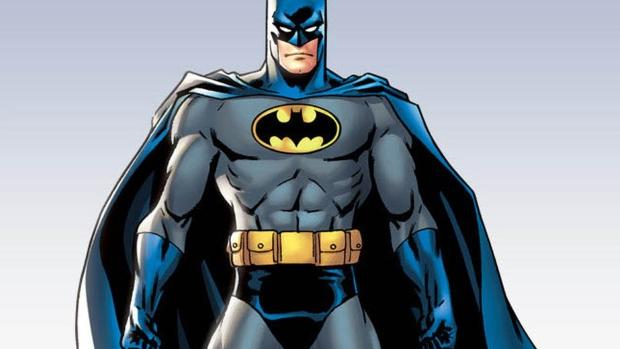
\includegraphics[width=\textwidth]{batman.jpg}
		}
	\caption{batman.jpg \label{fig:vaorig}}
	\end{subfigure}
	\hspace{5mm}
	\begin{subfigure}[b]{0.45\textwidth}
		\noindent\makebox[\textwidth]{
		  
\includegraphics[width=\textwidth]{seg_scrabbles.png}
		}
	\caption{Scribbles for the color histogram \label{fig:vadenoised}}
	\end{subfigure}
\end{figure}

\pagebreak

The segmentation result with $\lambda = 0.0075$ is as Figure \ref{fig:batmanseg} (after 2000 iterations). 

\begin{figure}[H]
\vspace{-5mm}
\caption{Segmentation result($\lambda = 0.0075$)\label{fig:batmanseg}}
\noindent\makebox[\textwidth]{
  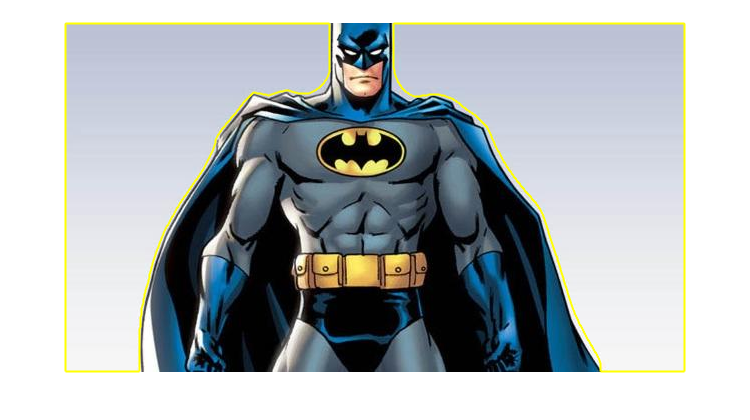
\includegraphics[width=\textwidth]{seg_result.png}
}
\end{figure}

\vspace{-5mm}
The segmentation result with different value of $\lambda$ is as follows:

\begin{figure}[H]
	\caption{Function x with different $\lambda$}
	\centering
	\begin{subfigure}[b]{0.30\textwidth}
		\noindent\makebox[\textwidth]{
		  
\includegraphics[width=\textwidth]{seg_x_0075}
		}
	\caption{$\lambda = 0.075$}
	\end{subfigure}
	\begin{subfigure}[b]{0.30\textwidth}
		\noindent\makebox[\textwidth]{
		  
\includegraphics[width=\textwidth]{seg_x.png}
		}
	\caption{$\lambda = 0.0075$}
	\end{subfigure}
	\begin{subfigure}[b]{0.30\textwidth}
		\noindent\makebox[\textwidth]{
		  
\includegraphics[width=\textwidth]{seg_x_000075.png}
		}
	\caption{$\lambda = 0.00075$}
	\end{subfigure}
\end{figure}


\subsection{Discussion}

\begin{itemize}
	\item Primal dual TV segmentation vs Graph-cuts
		\begin{itemize} 
			\item Primal dual TV segmentation is easy to parallelize thus faster on a multi cores. 
			\item Graph-cuts is faster on a single core.
			\item Primal dual TV treats image as continuous function, thus there's no metrication error. (discretization errors originated from the graph neighborhood)
			\item Primal dual TV is more memory efficient: it does not require graph structure.
			\item Graph-cuts is more intuitive: each nodes represent each pixels of a image. 
			\item Primal dual TV has mathematically clear formulation but more complex. 
			\item For graph-cuts, non-metric smoothness terms can be applied. 
		\end{itemize}
\end{itemize}

\pagebreak

%----------------------------------------------------------------------------------------
%	PROBLEM 3
%----------------------------------------------------------------------------------------

\section{Task 3: Applications of Inpainting}

\subsection{Description}

For recovering(inpainting) problem, cost function has the following form:

\begin{equation}
	G(x) = \frac{1}{2} \sum_{i, j \in \mathcal{D}_I \setminus \mathcal{I}} \frac{1}{2} (I_{i,j} - x_{i,j})
\end{equation}

where, $\mathcal{D}_I$ is the domain of 2D image $I$, and $\mathcal{I}$ is the set of all the missing pixels. \\

The primal dual algorithm is used to solve following equation: 

\begin{align}
	\min_{x \in X} \max_{y \in D_X} & \langle \nabla x, y \rangle + \lambda G(x) - \delta_Y (y) \notag \\
	&= \min_{x \in X} \max_{y \in D_X} \langle \nabla x, y \rangle + \frac{\lambda}{2} \sum_{i, j \in \mathcal{D}_I \setminus \mathcal{I}} \frac{1}{2} (I_{i,j} - x_{i,j}) - \delta_Y (y)  
\end{align}


%----------------------------------------------------------------------------------------
%	TASK 1
%----------------------------------------------------------------------------------------

\subsection{Task 1: Recovering an image with a high number of missing pixels}

\subsubsection{Results}

For this task, primal dual algorithm used for recovering damaged image which 90 \% of the pixels were removed.
\vspace{-5mm}
\begin{figure}[H]
	\caption{Original image and damaged image}
	\centering
	\begin{subfigure}[b]{0.45\textwidth}
		\noindent\makebox[\textwidth]{
		  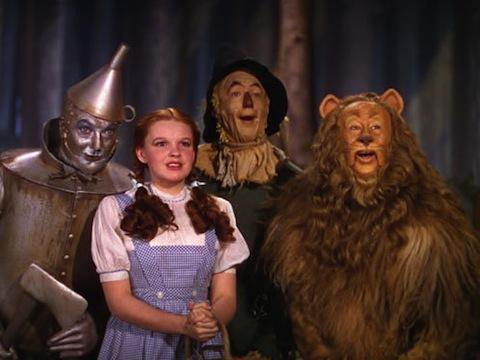
\includegraphics[width=\textwidth]{inp_orig.jpg}
		}
	\caption{Original image oz2.jpg}
	\end{subfigure}
	\hspace{5mm}
	\begin{subfigure}[b]{0.45\textwidth}
		\noindent\makebox[\textwidth]{
		  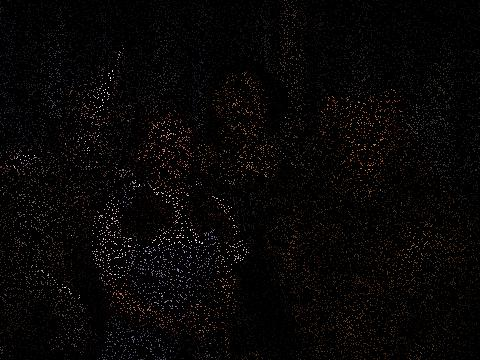
\includegraphics[width=\textwidth]{inp_removed.jpg}
		}
	\caption{Damaged image}
	\end{subfigure}
\end{figure}

As iteration goes on, damaged image is getting recovered. Figure \ref{fig:inpaint} shows the evolution of image with $\lambda = 5$.

\begin{figure}[H]
	\caption{Image evolution by inpainting\label{fig:inpaint}}
	\centering
	\begin{subfigure}[b]{0.3\textwidth}
		\noindent\makebox[\textwidth]{
		  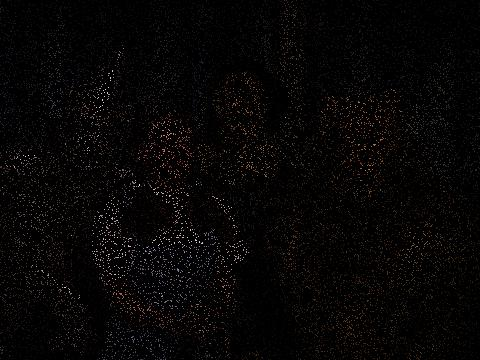
\includegraphics[width=\textwidth]{inp1.jpg}
		}
	\caption{iter $=1$}
	\end{subfigure}
	\begin{subfigure}[b]{0.3\textwidth}
		\noindent\makebox[\textwidth]{
		  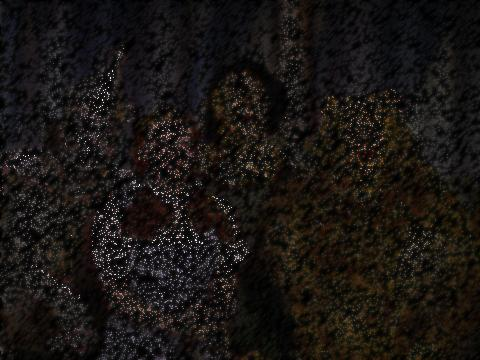
\includegraphics[width=\textwidth]{inp50.jpg}
		}
	\caption{iter $=50$}
	\end{subfigure}
		\begin{subfigure}[b]{0.3\textwidth}
		\noindent\makebox[\textwidth]{
		  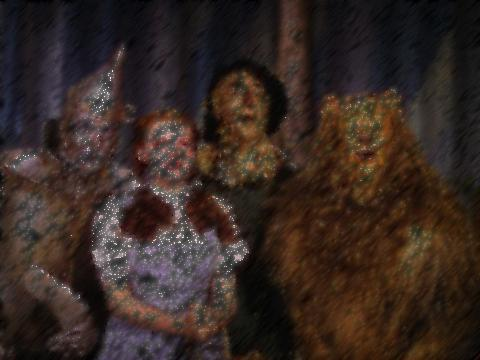
\includegraphics[width=\textwidth]{inp200.jpg}
		}
	\caption{iter $=200$}
	\end{subfigure}
	\begin{subfigure}[b]{0.3\textwidth}
		\noindent\makebox[\textwidth]{
		  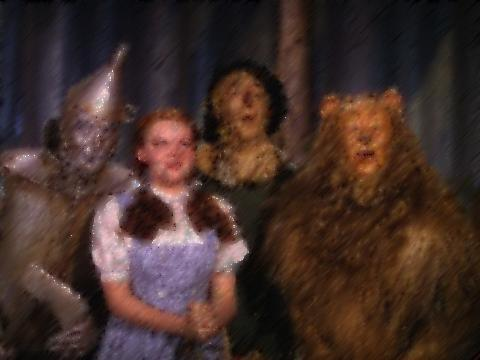
\includegraphics[width=\textwidth]{inp500.jpg}
		}
	\caption{iter $=500$}
	\end{subfigure}
	\begin{subfigure}[b]{0.3\textwidth}
		\noindent\makebox[\textwidth]{
		  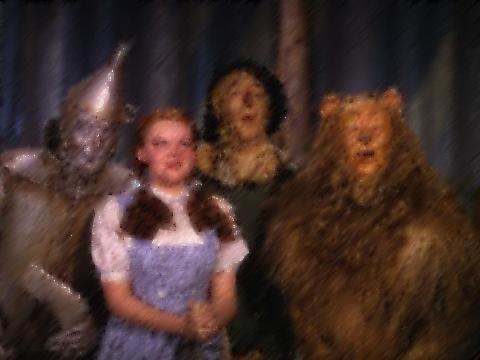
\includegraphics[width=\textwidth]{inp1000.jpg}
		}
	\caption{iter $=1000$}
	\end{subfigure}
	\begin{subfigure}[b]{0.3\textwidth}
		\noindent\makebox[\textwidth]{
		  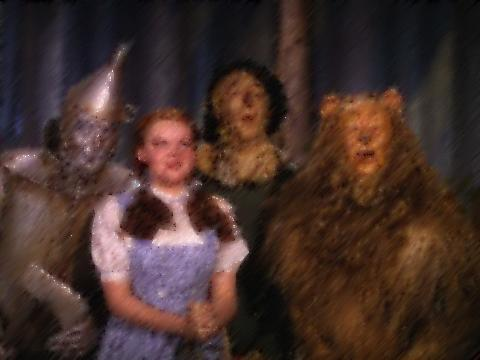
\includegraphics[width=\textwidth]{inp2000.jpg}
		}
	\caption{iter $=2000$}
	\end{subfigure}
\end{figure}

\vspace{-5mm}
\begin{figure}[H]
	\caption{Original image and final result}
	\centering
	\begin{subfigure}[b]{0.4\textwidth}
		\noindent\makebox[\textwidth]{
		  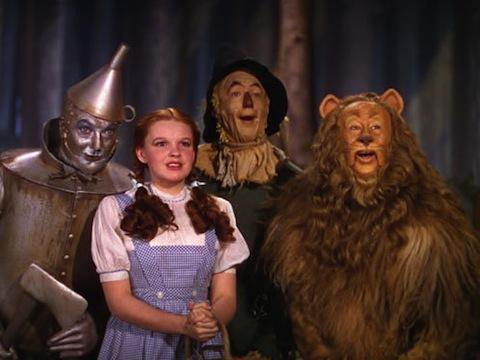
\includegraphics[width=\textwidth]{inp_orig.jpg}
		}
	\caption{Original image oz2.jpg}
	\end{subfigure}
	\hspace{5mm}
	\begin{subfigure}[b]{0.4\textwidth}
		\noindent\makebox[\textwidth]{
		  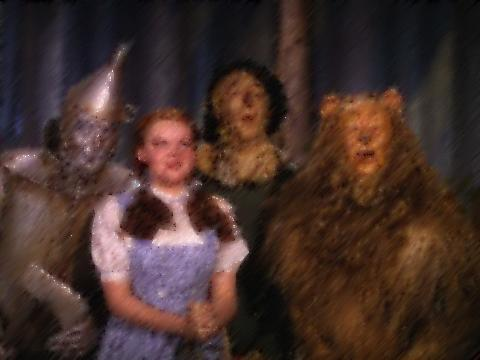
\includegraphics[width=\textwidth]{inp2000.jpg}
		}
	\caption{result of iter $=2000$}
	\end{subfigure}
\end{figure}

The result with different $\lambda$ is as Figure \ref{fig:inplambda}.
\vspace{-5mm}
\begin{figure}[H]
	\caption{Result with different $\lambda$ \label{fig:inplambda}}
	\centering
	\begin{subfigure}[b]{0.3\textwidth}
		\noindent\makebox[\textwidth]{
		  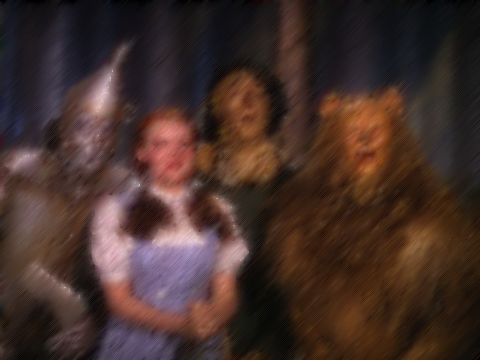
\includegraphics[width=\textwidth]{inp_lambda05.png}
		}
	\caption{$\lambda = 0.5$}
	\end{subfigure}
	\begin{subfigure}[b]{0.3\textwidth}
		\noindent\makebox[\textwidth]{
		  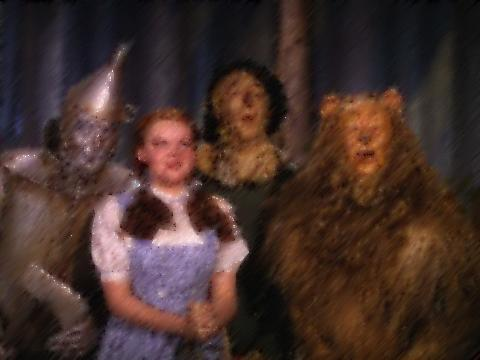
\includegraphics[width=\textwidth]{inp2000.jpg}
		}
	\caption{$\lambda = 5$}
	\end{subfigure}
	\begin{subfigure}[b]{0.3\textwidth}
		\noindent\makebox[\textwidth]{
		  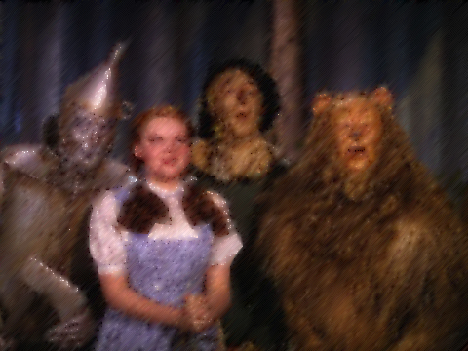
\includegraphics[width=\textwidth]{inp_lambda50.png}
		}
	\caption{$\lambda = 50$}
	\end{subfigure}
\end{figure}



%----------------------------------------------------------------------------------------
%	TASK 2
%----------------------------------------------------------------------------------------

\subsection{Task 2: Removing an object from an image}

\subsubsection{Results}

In this task, artifacts of the original image were removed and inpainted. Figure \ref{fig:lincoln} is original image with artifacts and scrabbles which indicates the region to be removed. 

\begin{figure}[H]
	\caption{Original image and damaged image \label{fig:lincoln}}
	\centering
	\begin{subfigure}[b]{0.32\textwidth}
		\noindent\makebox[\textwidth]{
		  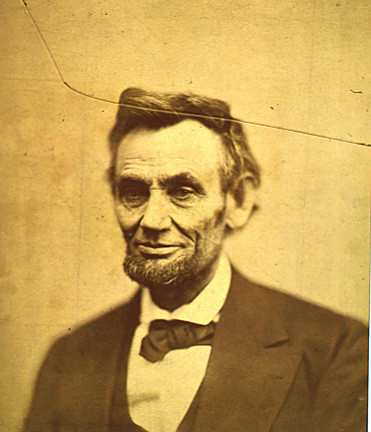
\includegraphics[width=\textwidth]{lincoln.jpg}
		}
	\caption{iter $=1$}
	\end{subfigure}
	\hspace{5mm}
	\begin{subfigure}[b]{0.32\textwidth}
		\noindent\makebox[\textwidth]{
		  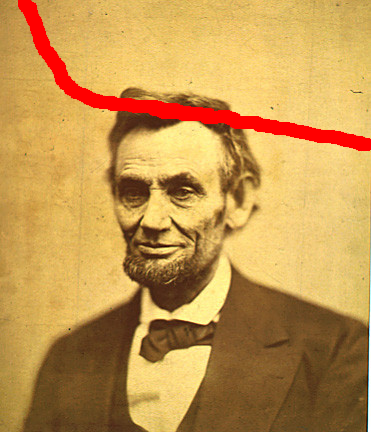
\includegraphics[width=\textwidth]{inpainter_scrabbles.png}
		}
	\caption{iter $=50$}
	\end{subfigure}
\end{figure}

After removing artifacts regions, the image is getting recovered as Figure \ref{fig:inpainter}.

\begin{figure}[H] 
	\caption{Image eveolution by inpainting \label{fig:inpainter}}
	\centering
	\begin{subfigure}[b]{0.22\textwidth}
		\noindent\makebox[\textwidth]{
		  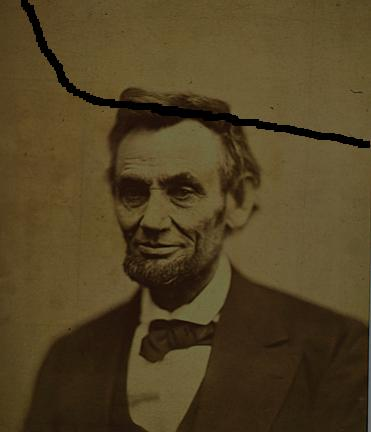
\includegraphics[width=\textwidth]{inpainter1.jpg}
		}
	\caption{iter $=1$}
	\end{subfigure}
	\begin{subfigure}[b]{0.22\textwidth}
		\noindent\makebox[\textwidth]{
		  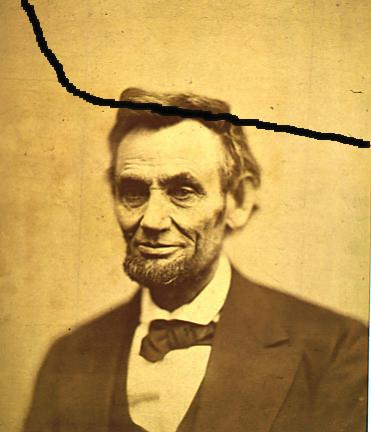
\includegraphics[width=\textwidth]{inpainter50.jpg}
		}
	\caption{iter $=50$}
	\end{subfigure}
	\begin{subfigure}[b]{0.22\textwidth}
		\noindent\makebox[\textwidth]{
		  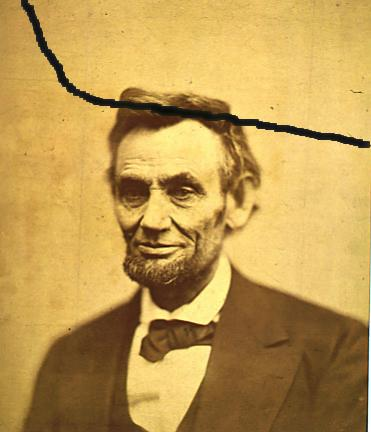
\includegraphics[width=\textwidth]{inpainter100.jpg}
		}
	\caption{iter $=100$}
	\end{subfigure}
	\begin{subfigure}[b]{0.22\textwidth}
		\noindent\makebox[\textwidth]{
		  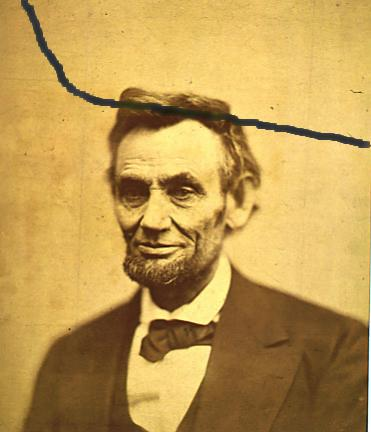
\includegraphics[width=\textwidth]{inpainter200.jpg}
		}
	\caption{iter $=200$}
	\end{subfigure}
	\begin{subfigure}[b]{0.22\textwidth}
		\noindent\makebox[\textwidth]{
		  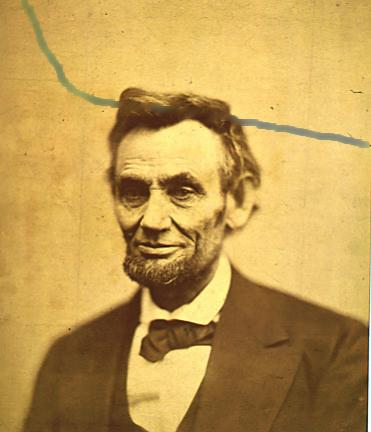
\includegraphics[width=\textwidth]{inpainter500.jpg}
		}
	\caption{iter $=500$}
	\end{subfigure}
	\begin{subfigure}[b]{0.22\textwidth}
		\noindent\makebox[\textwidth]{
		  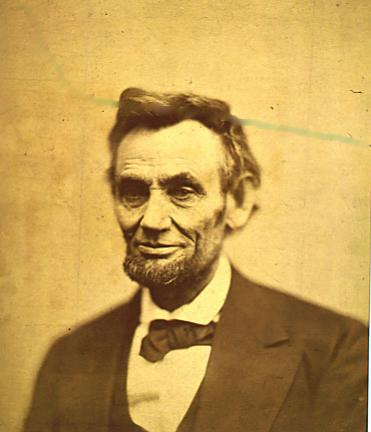
\includegraphics[width=\textwidth]{inpainter750.jpg}
		}
	\caption{iter $=750$}
	\end{subfigure}
	\begin{subfigure}[b]{0.22\textwidth}
		\noindent\makebox[\textwidth]{
		  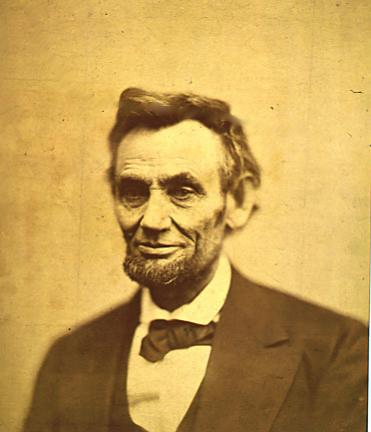
\includegraphics[width=\textwidth]{inpainter1000.jpg}
		}
	\caption{iter $=1000$}
	\end{subfigure}
	\begin{subfigure}[b]{0.22\textwidth}
		\noindent\makebox[\textwidth]{
		  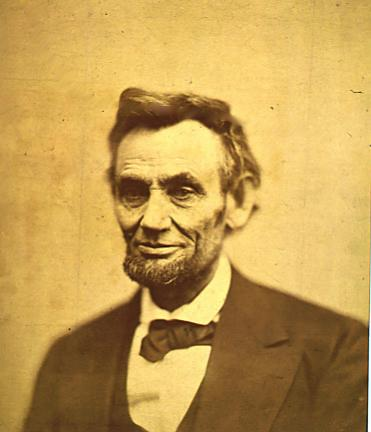
\includegraphics[width=\textwidth]{inpainter2000.jpg}
		}
	\caption{iter $=2000$}
	\end{subfigure}
\end{figure}

\begin{figure}[H]
	\caption{Original image and recovered image \label{fig:lincoln}}
	\centering
	\begin{subfigure}[b]{0.45\textwidth}
		\noindent\makebox[\textwidth]{
		  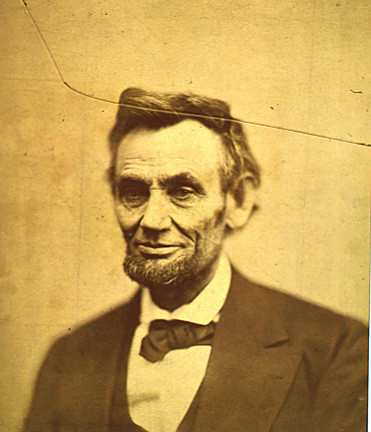
\includegraphics[width=\textwidth]{lincoln.jpg}
		}
	\caption{lincoln.jpg}
	\end{subfigure}
	\hspace{5mm}
	\begin{subfigure}[b]{0.45\textwidth}
		\noindent\makebox[\textwidth]{
		  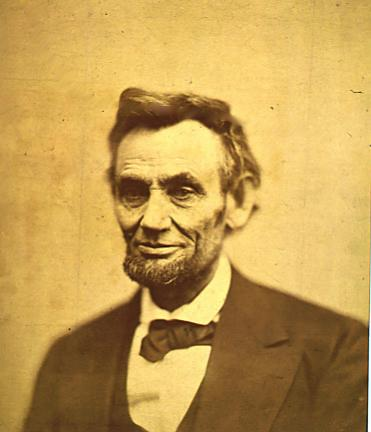
\includegraphics[width=\textwidth]{inpainter2000.jpg}
		}
	\caption{result of iter $=2000$}
	\end{subfigure}
\end{figure}

%----------------------------------------------------------------------------------------
%\subsection{Discussion}



%----------------------------------------------------------------------------------------
%	REFERENCES
%----------------------------------------------------------------------------------------

%\bibliography{reference} 
%\bibliographystyle{ieeetr}

\end{document}
